\testfile{pgfplotstest.plottypes.tex}
\testsection{Stacked plots}
%\tikzstyle{every axis}+=[reverse stacked plots=false]
\testsubsection{stack y, sharp plot}
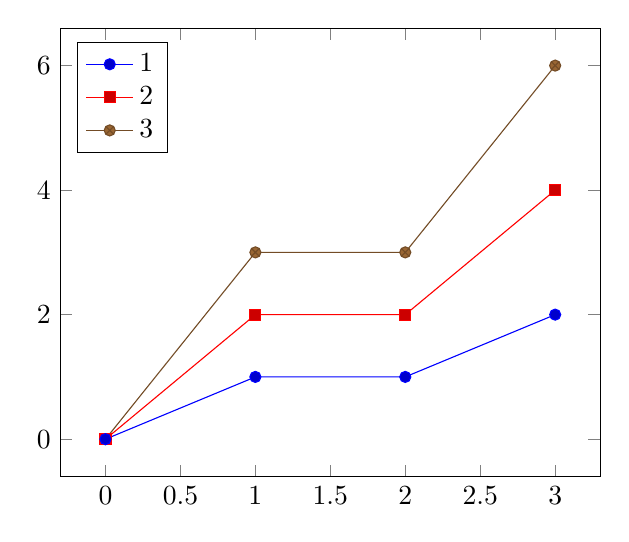
\begin{tikzpicture}
%\tracingmacros=2\tracingcommands=2
	\begin{axis}[stack plots=y,
		legend style={at={(0.03,0.97)},anchor=north west}
	]
	\addplot coordinates {(0,0) (1,1) (2,1) (3,2)};
	\addplot coordinates {(0,0) (1,1) (2,1) (3,2)};
	\addplot coordinates {(0,0) (1,1) (2,1) (3,2)};
	\legend{1,2,3}%
	\end{axis}
%\tracingmacros=0\tracingcommands=0
\end{tikzpicture}

\testsubsubsection{with closedcycle}
\begingroup
\def\example#1{%
\begin{tikzpicture}
	\begin{axis}[stack plots=y,
		legend style={at={(0.03,0.97)},anchor=north west}
	]
	\addplot+[#1] coordinates {(0,0) (1,1) (2,1) (3,2)} \closedcycle;
	\addplot+[#1] coordinates {(0,0) (1,1) (2,1) (3,2)} \closedcycle;
	\addplot+[#1] coordinates {(0,0) (1,1) (2,1) (3,2)} \closedcycle;
	\legend{1,2,3}%
	\end{axis}
\end{tikzpicture}
}

\example{}

\example{fill}
\endgroup

\testsubsubsection{with closedcycle and const plots}
\begingroup
\def\example#1{%
\begin{tikzpicture}[#1]
	\begin{axis}[stack plots=y,
		legend style={at={(0.03,0.97)},anchor=north west}
	]
	\addplot+[fill] coordinates {(0,0.5) (1,1) (2,1) (3,2) (4,2)}  \closedcycle;
	\addplot+[fill] coordinates {(0,0.5) (1,1) (2,1) (3,2) (4,2)} \closedcycle;
	\addplot+[fill] coordinates {(0,0.5) (1,1) (2,1) (3,2) (4,2)} \closedcycle;
	\legend{1,2,3}%
	\end{axis}
\end{tikzpicture}
}

\example{const plot mark left}

\example{const plot mark right}
\endgroup

\testsubsection{stack y, ybar}
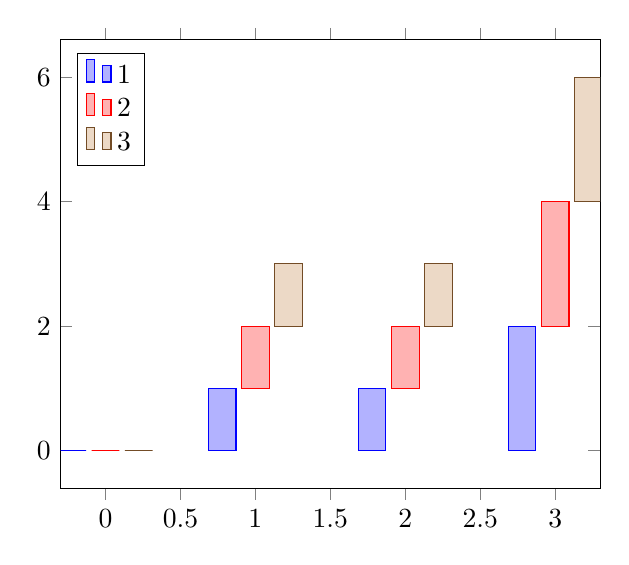
\begin{tikzpicture}
	\begin{axis}[stack plots=y,
		ybar,
		legend style={at={(0.03,0.97)},anchor=north west},
	]
	\addplot coordinates {(0,0) (1,1) (2,1) (3,2)};
	\addplot coordinates {(0,0) (1,1) (2,1) (3,2)};
	\addplot coordinates {(0,0) (1,1) (2,1) (3,2)};
	\legend{1,2,3}%
	\end{axis}
\end{tikzpicture}

\testsubsection{stack y, ybar, minus}
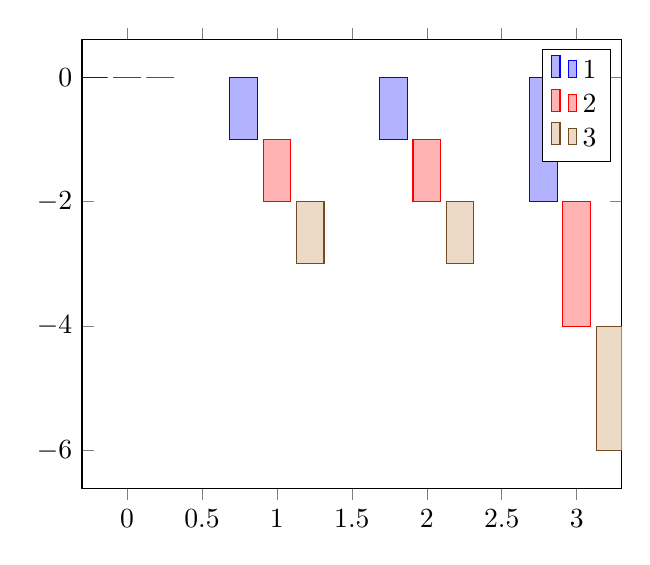
\begin{tikzpicture}
	\begin{axis}[stack plots=y,stack dir=minus,
		ybar,
	]
	\addplot coordinates {(0,0) (1,1) (2,1) (3,2)};
	\addplot coordinates {(0,0) (1,1) (2,1) (3,2)};
	\addplot coordinates {(0,0) (1,1) (2,1) (3,2)};
	\legend{1,2,3}%
	\end{axis}
\end{tikzpicture}

\testsubsection{stack x, sharp plot [not useful]}
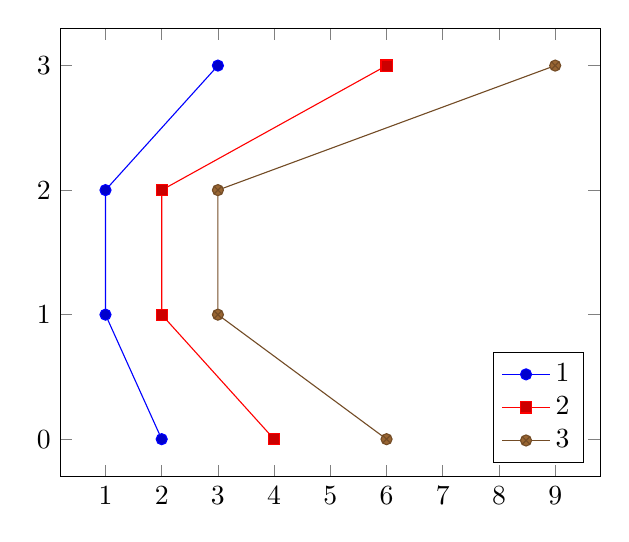
\begin{tikzpicture}
%\tracingmacros=2\tracingcommands=2
	\begin{axis}[stack plots=x,
		legend style={at={(0.97,0.03)},anchor=south east},
		xtick={0,...,30},
	]
	\addplot coordinates {(2,0) (1,1) (1,2) (3,3)};
	\addplot coordinates {(2,0) (1,1) (1,2) (3,3)};
	\addplot coordinates {(2,0) (1,1) (1,2) (3,3)};
	\legend{1,2,3}%
	\end{axis}
%\tracingmacros=0\tracingcommands=0
\end{tikzpicture}

\testsubsection{stack x, xbar}
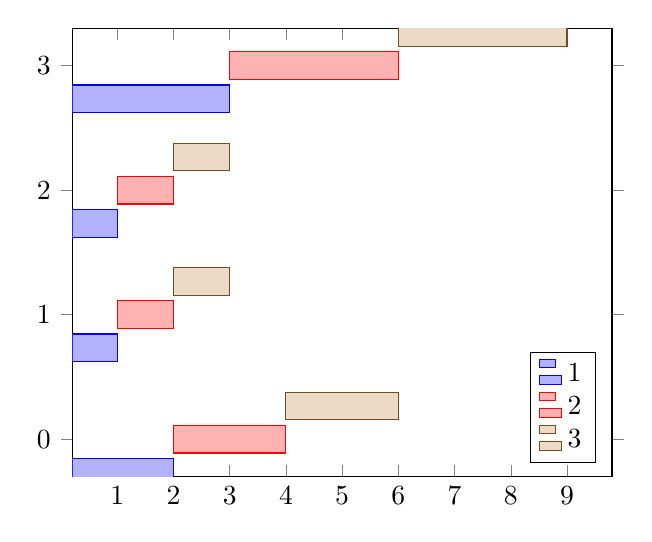
\begin{tikzpicture}
	\begin{axis}[stack plots=x,
		xbar,
		xtick={0,...,30},
		legend style={at={(0.97,0.03)},anchor=south east},
	]
	\addplot coordinates {(2,0) (1,1) (1,2) (3,3)};
	\addplot coordinates {(2,0) (1,1) (1,2) (3,3)};
	\addplot coordinates {(2,0) (1,1) (1,2) (3,3)};
	\legend{1,2,3}%
	\end{axis}
\end{tikzpicture}

\testsubsection{stack x, xbar, minus}
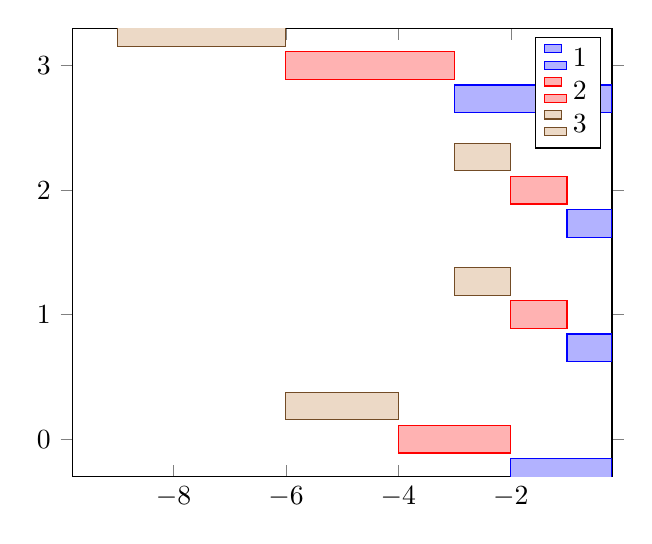
\begin{tikzpicture}
	\begin{axis}[stack plots=x,
		stack dir=minus,
		xbar,
	]
	\addplot coordinates {(2,0) (1,1) (1,2) (3,3)};
	\addplot coordinates {(2,0) (1,1) (1,2) (3,3)};
	\addplot coordinates {(2,0) (1,1) (1,2) (3,3)};
	\legend{1,2,3}%
	\end{axis}
\end{tikzpicture}

\testsection{Bar diagrams}
{
\pgfkeys{/pgfplots/bar style/.style={%
		%legend style={cells={anchor=base}},
		/pgfplots/legend image code/.code={\draw[##1,yshift=-0.2em] plot coordinates {(0cm,0.8em) (11pt,0.6em)};},
		/tikz/every axis plot/.style={
			xshift={%
				% total width = n*w + (n-1)*skip
				% -> subtract half for centering
				-0.5*(\numplots*\pgfplotbarwidth + (\numplots-1)*2pt)  + 
				% the '0.5*w' is for centering
				(.5+\plotnum)*\pgfplotbarwidth + \plotnum*2pt}},%
	}
}%
\begin{tikzpicture}
	\begin{axis}[
		%xmin=1925,xmax=1975,disabledatascaling=false,
		%xtick={1930,1940,1950,1960,1970},
		tick align=outside,
		x tick label style={/pgf/number format/set thousands separator=},
		ylabel=Population,
		enlargelimits=0.15,
		legend style={at={(0.5,-0.1)},anchor=north,legend columns=-1},
		bar style,
	]
%\tracingmacros=2\tracingcommands=2
	\addplot[ybar,draw=blue,mark=none,fill=blue!80!black] 
		plot coordinates {(1930,50e6) (1940,33e6) (1950,40e6) (1960,50e6) (1970,70e6)};
	\addlegendentry[bar style]{FarFarAway}

	\addplot[ybar,mark=none,red,fill=red!80!black] 
		plot coordinates {(1930,38e6) (1940,42e6) (1950,43e6) (1960,45e6) (1970,65e6)};
	\addlegendentry[bar style]{NotSoFar}

	\addplot[ybar,mark=none,brown,fill=brown!80!black] 
		plot coordinates {(1930,15e6) (1940,12e6) (1950,13e6) (1960,25e6) (1970,35e6)};
	\addlegendentry[bar style]{Near}
	\end{axis}
\end{tikzpicture}

\testsubsection{Interval bar handlers}
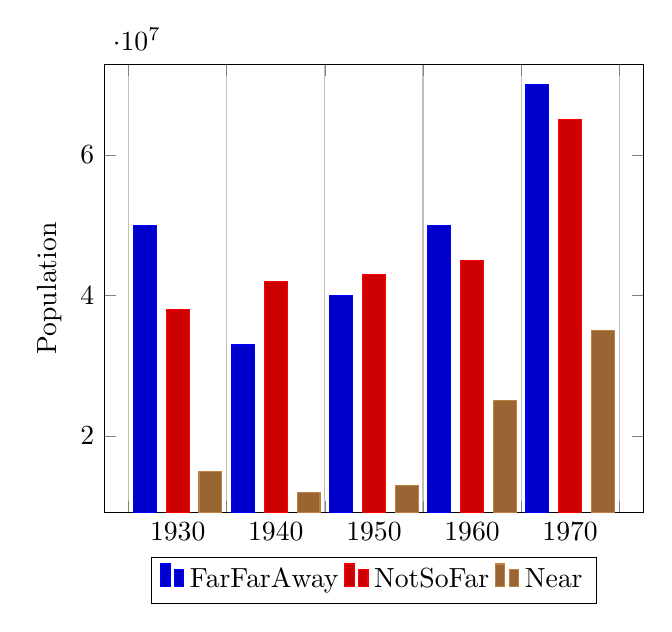
\begin{tikzpicture}
	\begin{axis}[
		x tick label style={/pgf/number format/set thousands separator=},
		x tick label as interval,
		ylabel=Population,
		enlargelimits=0.05,
		xmajorgrids,
		/pgfplots/legend image code/.code={\draw[#1,yshift=-0.2em,bar interval width=0.7,bar interval shift=0.5] plot coordinates {(0cm,0.8em) (5pt,0.6em) (10pt,0.6em)};},
		legend style={at={(0.5,-0.1)},anchor=north,legend columns=-1},
		bar interval width=0.7/\numplots,
		bar interval shift={(\plotnum+0.5)/\numplots},
	]
	\addplot[ybar interval,draw=blue,mark=none,fill=blue!80!black]
		plot coordinates {(1930,50e6) (1940,33e6) (1950,40e6) (1960,50e6) (1970,70e6) (1980,70e6)};
	\addlegendentry{FarFarAway}

	\addplot[ybar interval,mark=none,red,fill=red!80!black] 
		plot coordinates {(1930,38e6) (1940,42e6) (1950,43e6) (1960,45e6) (1970,65e6) (1980,70e6)};
	\addlegendentry{NotSoFar}

	\addplot[ybar interval,mark=none,brown,fill=brown!80!black] 
		plot coordinates {(1930,15e6) (1940,12e6) (1950,13e6) (1960,25e6) (1970,35e6) (1980,70e6)};
	\addlegendentry{Near}
	\end{axis}
\end{tikzpicture}



\testsection{const plot}
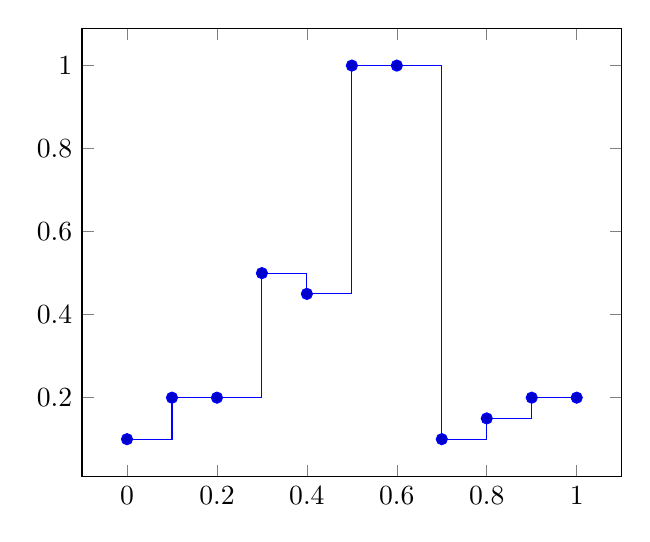
\begin{tikzpicture}
	\begin{axis}
	\addplot+[const plot]
		coordinates {(0,0.1) (0.1,0.2) (0.2,0.2) (0.3,0.5) (0.4,0.45) (0.5,1) (0.6,1) (0.7,0.1) (0.8,0.15) (0.9,0.2) (1,0.2)};
	\end{axis}
\end{tikzpicture}

\testsection{const plot mark right}
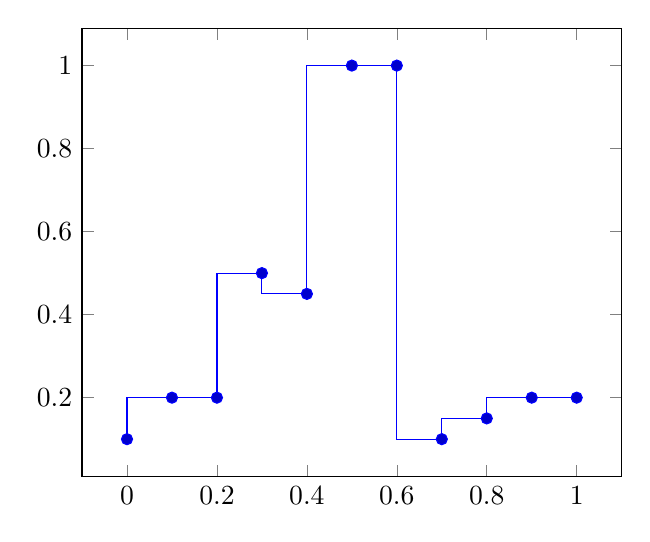
\begin{tikzpicture}
	\begin{axis}
	\addplot+[const plot mark right]
		coordinates {(0,0.1) (0.1,0.2) (0.2,0.2) (0.3,0.5) (0.4,0.45) (0.5,1) (0.6,1) (0.7,0.1) (0.8,0.15) (0.9,0.2) (1,0.2)};
	\end{axis}
\end{tikzpicture}

\testsection{jump mark right}
\begin{tikzpicture}
	\begin{axis}
	\addplot+[jump mark right]
		coordinates {(0,0.1) (0.1,0.2) (0.2,0.2) (0.3,0.5) (0.4,0.45) (0.5,1) (0.6,1) (0.7,0.1) (0.8,0.15) (0.9,0.2) (1,0.2)};
	\end{axis}
\end{tikzpicture}

\testsection{jump mark left}
\begin{tikzpicture}
	\begin{axis}
	\addplot+[jump mark left]
		coordinates {(0,0.1) (0.1,0.2) (0.2,0.2) (0.3,0.5) (0.4,0.45) (0.5,1) (0.6,1) (0.7,0.1) (0.8,0.15) (0.9,0.2) (1,0.2)};
	\end{axis}
\end{tikzpicture}
